\documentclass[class=report, crop=false, 12pt,a4paper]{standalone}
\usepackage{enumitem}
\usepackage{multicol}
\usepackage{graphicx}
\usepackage{float}
\usepackage{amsmath}
\usepackage{amssymb}
\usepackage{mathtools}
\usepackage{siunitx}
\usepackage{commath}
\usepackage{array}
\usepackage{natbib}
\usepackage[a4paper,width=150mm,top=25mm,bottom=25mm]{geometry}
\setlength{\parindent}{0pt}
\begin{document}
\begin{center}
  20/11/2020
\end{center}
What you already know on bending is sufficient to enable the basic engineering design of static beam structures. Basic engineering design is primarily concerned with:
\begin{itemize}
  \item Controlling elastic deformations
  \item Maintaining structures within their elastic range
\end{itemize}
However, for safety reasons, it is essental for engineers to be able to predict how a structure would fail if unexpected loading condiitons occur. 
\section{Introduction}
\subsection{Elastic and Plastic Regimes}
Stressing within the \textbf{elastic regime}:
\begin{itemize}
  \item Material returns to original state upon removal of external actions
  \item Deformation depends solely upon stress and not upon load history
\end{itemize}
Exceeding the elastic regime, \textbf{plastic regime} is reached:
\begin{itemize}
  \item Permanent distortions take place in the material
  \item Deformation depends upon stress and load history
\end{itemize}
Equations of solid mechanics apply to both cases.
\begin{figure}[H]
  \centering
  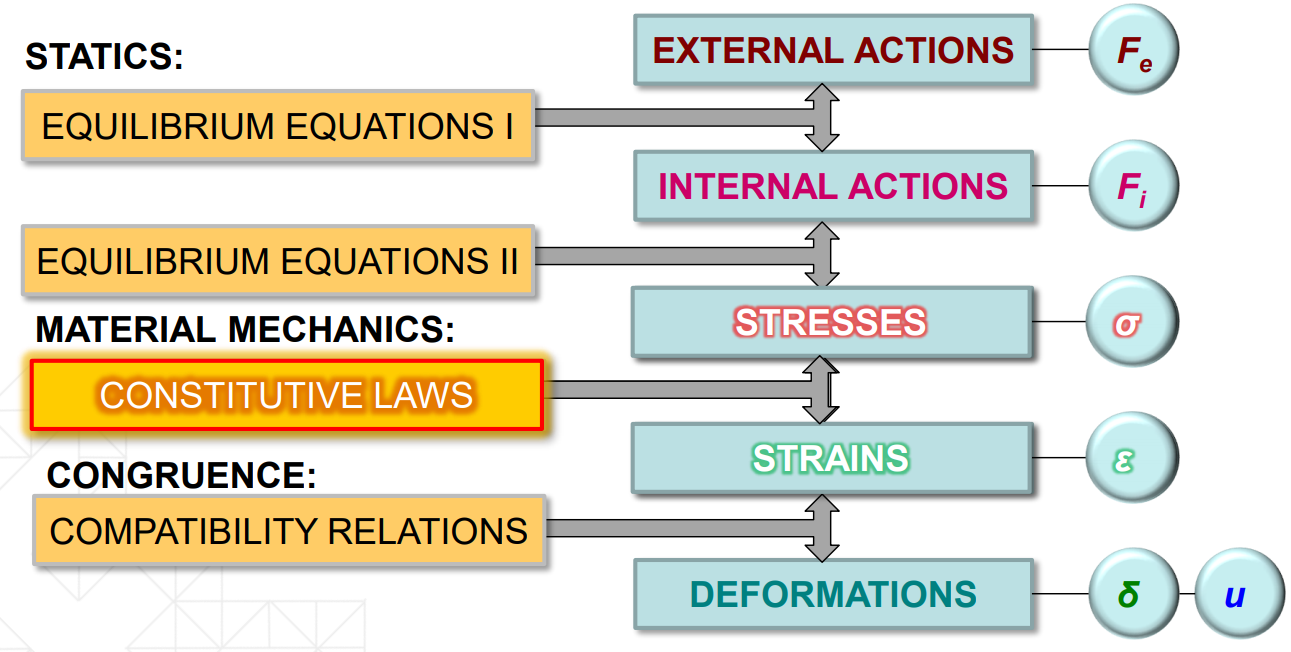
\includegraphics[width = 0.7 \textwidth]{../img/diagram1.PNG}
  \caption{Solid Mechanics Equations: The relationship between actions, stresses, strains and deformations}
\end{figure}
\subsection{Stress-Strain Plastic Relationship}
\begin{figure}[H]
  \centering
  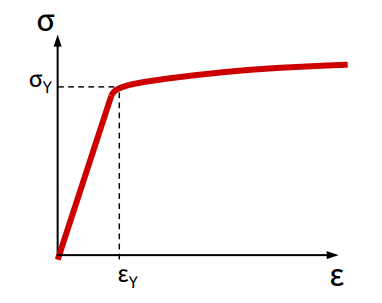
\includegraphics[width = 0.4 \textwidth]{../img/graph4.PNG}
  \caption{Typical elasto-plastic material}
\end{figure}
Typical elasto-plastic material:
\begin{itemize}
  \item Region 1 - linear elastic behaviour up to yield stress $\sigma_y$
  \item Region 2 – non linear development with strain-hardening
\end{itemize}
\begin{figure}[H]
  \centering
  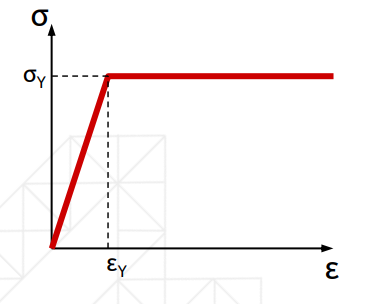
\includegraphics[width = 0.4 \textwidth]{../img/graph5.PNG}
  \caption{Perfectly elasto-plastic material}
\end{figure}
Perfectly elasto-plastic material:
\begin{itemize}
  \item Region 1 - linear elastic behaviour up to yield stress $\sigma_y$
  \item Region 2 – strain increases at constant stress
\end{itemize}
\textbf{Structural steels} are elastoplastic materials and can be modelled as perfectly elastoplastic (neglecting the strain-hardening is conservative for safety).
\section{Plastic Theory of Collapse}
\subsection{Bending and Plastic Collapse}
\textbf{Bending moment} is by far the most relevant of the internal forces, since it produces the largest levels of deformations and stress into the beam. Therefore, \textbf{plastic collapse} of beam structures is commonly associated with \textbf{plastic bending}.
Assumptions: 
\begin{itemize}
  \item Material is perfectly elasto-plastic. (in the plastic region stress will be constant)
  \item Yield stress is the same in tension and compression
  \item Transverse cross-sections remain plane (strain is proportional to the distance from the NA)
  \item When a cross-section is fully plastic (plastic hinge), its resisting moment remains constant until collapse of the whole structure
  \item Loads increase monotonically
\end{itemize}
\subsection{Elastic Bending Moment}
Consider a beam of rectangular cross-section, subjected to pure bending.
\begin{figure}[H]
  \centering
  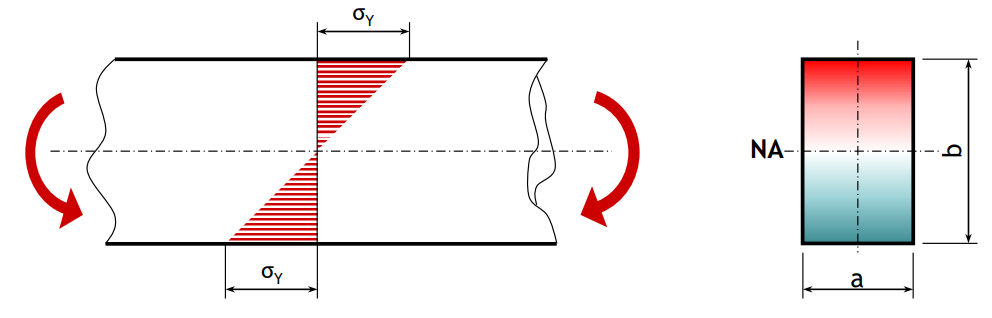
\includegraphics[width = 0.9 \textwidth]{../img/beam14.PNG}
\end{figure}
Maximum stress reaches the elastic limit $\sigma_y$ when the bending moment is equal to:
\begin{gather}
  M = \frac{EI}{R} \\
  \sigma = \frac{Eb}{2R} \\
  I = \frac{ab^3}{12} \\
  \therefore \text{The yield bending moment}: M_Y = \sigma_Y\frac{ab^2}{6}
\end{gather}
At the elastic moment, all fibres are still in the elastic condition. 
If moment increases further, external fibres exceed the elastic limit and yield: deformation increases but stress keeps constant and equal to $\sigma_y$. 
With increasing bending moment, the plastic region penetrates deeper toward the Neutral Axis (NA).
\subsection{Elasto-Plastic Bending Moment}
Consider a beam of rectangular cross-section, subjected to pure bending.
\begin{figure}[H]
  \centering
  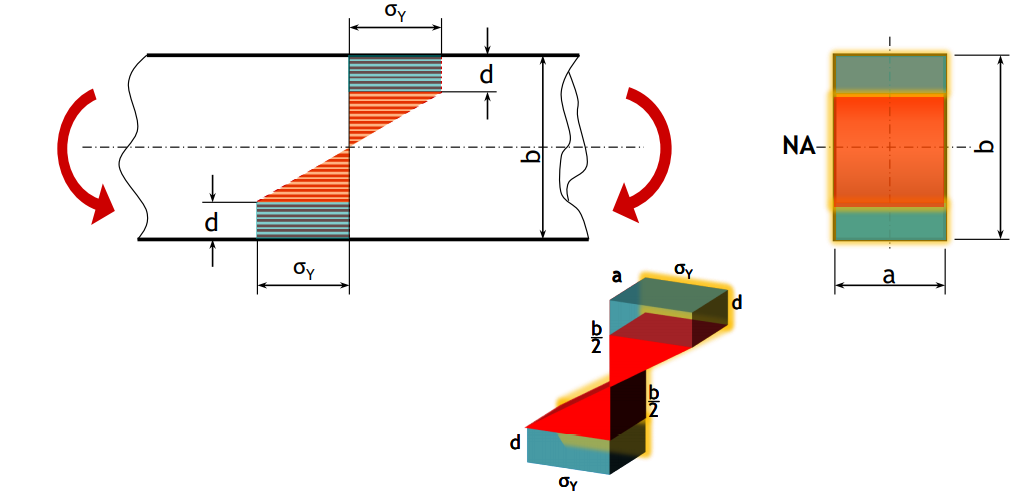
\includegraphics[width = 0.9 \textwidth]{../img/beam15.PNG}
\end{figure}
The moment is given by:
\begin{gather}
  M = \frac{\sigma I}{h} \\
  I = ? \\
  \therefore \text{Elasto-plastic bending moment}: M = \frac{\sigma_Y ab^2}{6}\left[1+2\frac{d}{b}\left(1-\frac{d}{b}\right)\right]
\end{gather}
\textbf{The derivation of the bending moment:}
\begin{figure}[H]
  \centering
  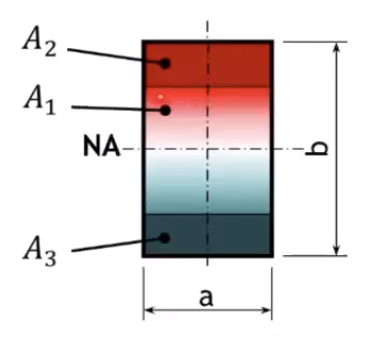
\includegraphics[width = 0.3 \textwidth]{../img/beam16.PNG}
\end{figure}
The cross-section is divided into 3 parts:
\begin{enumerate}
  \item Elastic part in the middle $(A_1)$
  \item Plastic part at the top $(A_2)$
  \item Plastic part at the bottom $(A_3)$
\end{enumerate}
\begin{gather}
  M = \int_{A}\dif M = \int_{A}h\cdot \sigma \dif A \\[10pt]
  = \int_{A_1}\frac{\sigma_Y h}{b/2-d}h\dif A + \int_{A_2}\sigma_Y h\dif A + \int_{A_3}\sigma_Y h\dif A \\[10pt]
  = \int_{-b/2+d}^{b/2-d}\frac{\sigma_Y a}{b/2-d}h^2\dif h + \int_{b/2-d}^{b/2}\sigma_Y ah\dif h + \int_{-b/2}^{-b/2+d}\sigma_Y ah\dif h \\[10pt]
  = \frac{\sigma_Y ab^2}{6}\left[1+2\frac{d}{b}\left(1-\frac{d}{b}\right)\right] 
\end{gather}
\subsection{Plastic Bending Moment}
Consider a beam of rectangular cross-section, subjected to pure bending.
\begin{figure}[H]
  \centering
  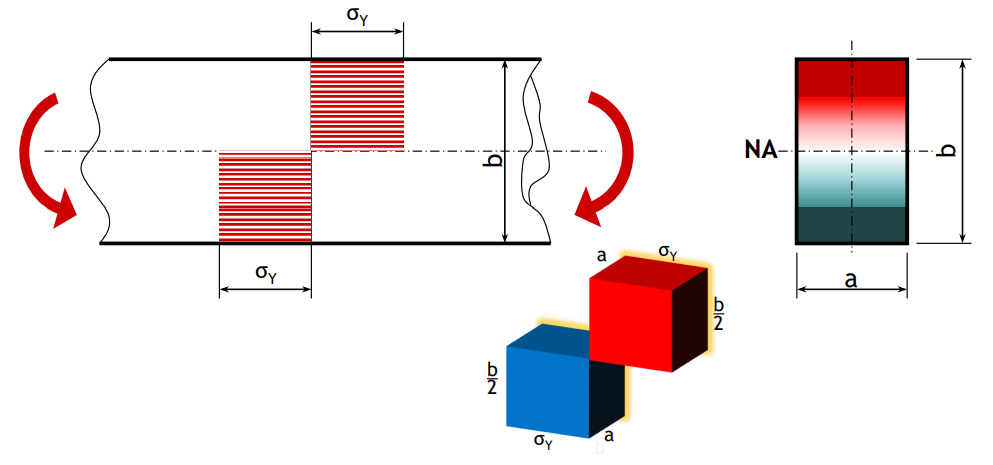
\includegraphics[width = 0.9 \textwidth]{../img/beam17.PNG}
\end{figure}
If bending moment keeps increasing, the plastic region propagate to the NA. In this case the moment is equal to:
\begin{gather}
  \text{Plastic bending moment}: M_P = \sigma_Y\frac{ab^2}{4}
\end{gather}
In practice, the plastic moment is given by the product of the yield stress by (the 1st moment of area (of the cross section) above the plastic NA + the 1st moment of area below the plastics NA).
\subsection{Shape Factor}
The yielding and plastic bending moments are different. In this case (rectangular cross-section) they are:
\begin{gather}
  M_Y = \sigma_Y\frac{ab^2}{6} \ \ \ \ \ M_P = \sigma_Y\frac{ab^2}{4}
\end{gather}
The ratio $f = \frac{M_P}{M_Y}$ between the yielding bending moment and the plastic bending moment is solely a function of the shape of the cross-section, and it is called \textbf{shape factor}. In this case (rectangular cross-section) it is:
\begin{gather}
  f = \frac{M_P}{M_Y} = \frac{\sigma_Y ab^2}{4}\frac{6}{\sigma_Y ab^2} = 1.5
\end{gather}
The shape factor is an indicator of the reserve strength that the beam can offer after yielding first begins.
\subsection{Plastic Collapse Under Bending}
\begin{figure}[H]
  \centering
  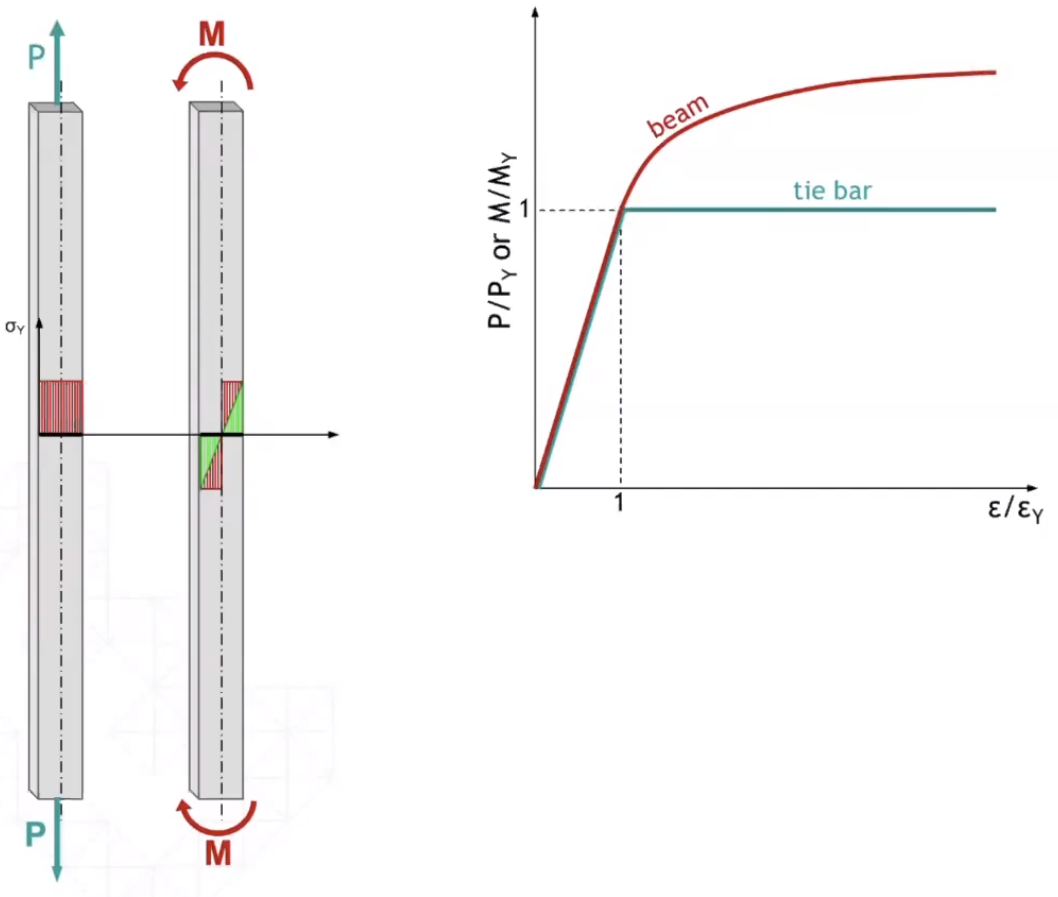
\includegraphics[width = 0.7 \textwidth]{../img/diagram2.PNG}
\end{figure}
Contrary to the case of normal load, the plastic collapse of a beam under pure bending occurs at a moment greater than the yield moment. \\\\
For a rectangular cross section, it will occur at a moment 50\% higher than the one that initiate yielding. 
\subsection{Neutral Axis with Asymmetry}
In the case of asymmetrical sections (though still singly symmetric), the analysis becomes more complex:
\begin{figure}[H]
  \centering
  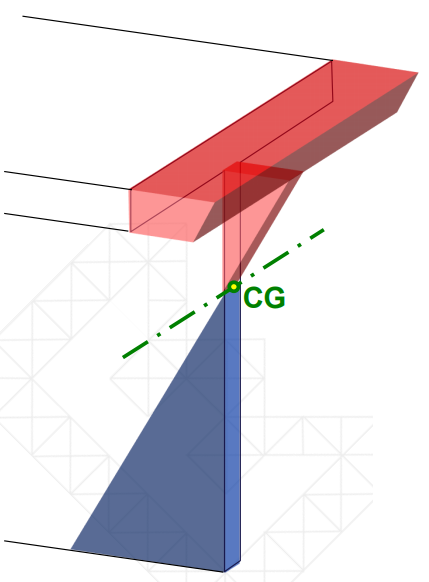
\includegraphics[width = 0.35 \textwidth]{../img/beam18.PNG}
\end{figure}
Equilibrium of forces in the ELASTIC case:
\begin{gather}
  F = \int_{A}\sigma\cdot\dif A = \int_{A}\frac{M}{I}h\cdot\dif A = \frac{M}{I}\int_{A}h\cdot\dif A = 0
\end{gather}
The $\int_{A}h\cdot\dif A$ is the 1st moment of area. The \textbf{elastic neutral axis} corresponds to the centroid of the section (centre of gravity).
\begin{figure}[H]
  \centering
  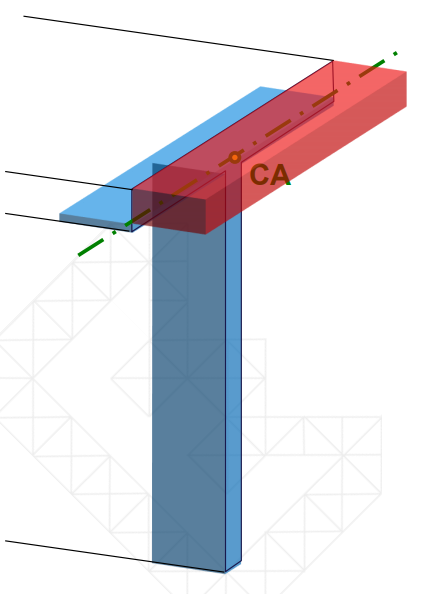
\includegraphics[width = 0.35 \textwidth]{../img/beam19.PNG}
\end{figure}
Equilibrium of forces in the PLASTIC case:
\begin{gather}
  F = \int_{A}\sigma_Y\cdot\dif A = \int_{A_T}\sigma_Y\cdot\dif A - \int_{A_C}\sigma_Y\cdot\dif A = 0 \\
  \therefore \sigma_Y A_T = \sigma_Y A_C \\
  \therefore A_T = A_C
\end{gather}
The \textbf{plastic neutral axis} corresponds to the centre of area (belongs to the line that divides the section into 2 equal areas).
\begin{figure}[H]
  \centering
  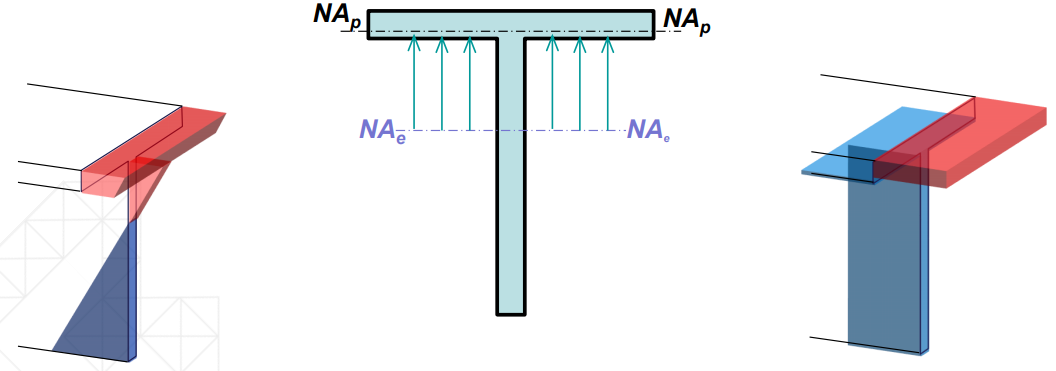
\includegraphics[width = 0.9 \textwidth]{../img/beam20.PNG}
  \caption{In the elasto-plastic phase, the neutral axis shifts from the centroid (centre of gravity) to the centre of area of the section}
\end{figure}
\subsection{Example: Shape factor for T-beam}
\begin{figure}[H]
  \centering
  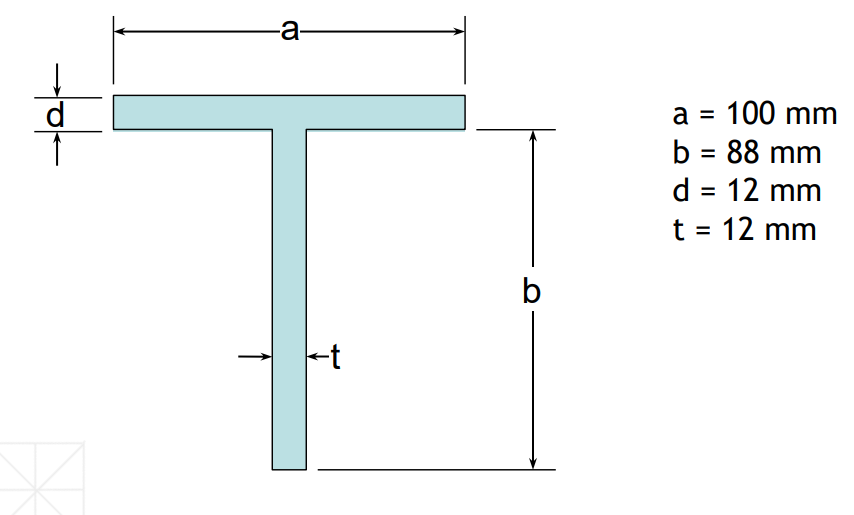
\includegraphics[width = 0.5 \textwidth]{../img/diagram3.PNG}
\end{figure}
Yield moment $M_Y$ and plastic moment $M_P$ need to be calculated:
\begin{gather}
  M_Y = \frac{\sigma_Y\cdot I}{h_{max}} \\
  M_P = \sigma_Y(Q_1+Q_2)
\end{gather}
\subsubsection{Elastic Neutral Axis:}
\begin{figure}[H]
  \centering
  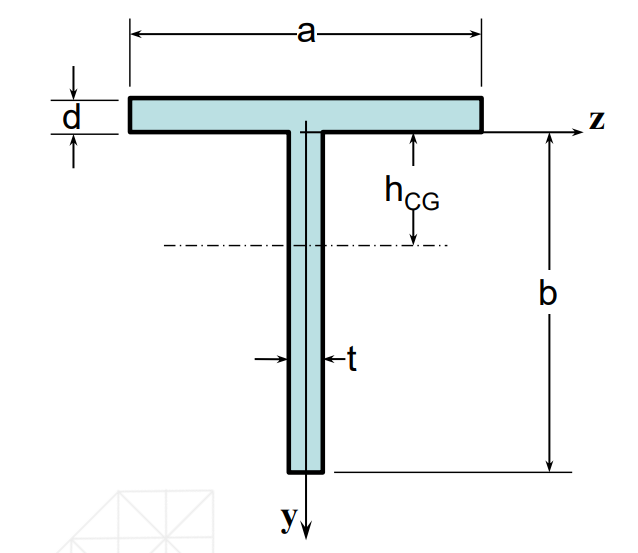
\includegraphics[width = 0.4 \textwidth]{../img/diagram4.PNG}
\end{figure}
\begin{gather}
  \text{Centre of Gravity} = h_{CG} = \frac{\int_{A}h\cdot\dif A}{A}
\end{gather}
\subsubsection{2nd Moment of Area:}
\begin{figure}[H]
  \centering
  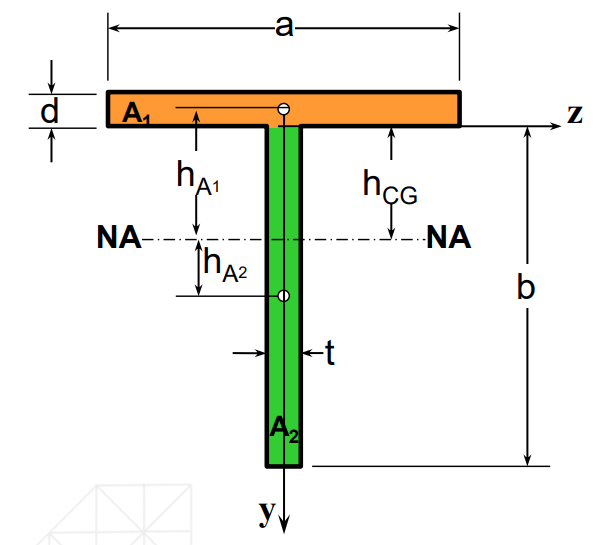
\includegraphics[width = 0.4 \textwidth]{../img/diagram5.PNG}
\end{figure}
\begin{gather}
  h_{A1} = h_{CG}+\frac{d}{2} = 23.4 \text{mm} \\
  h_{A2} = \frac{b}{2}-h_{CG} = -26.6 \text{mm}
\end{gather}
2nd moment of area (parallel axis theorem):
\begin{gather}
  I_{zz} = (I_{A_1}+A_1\cdot h_{A_1}^2)+(I_{A_2}+A_2\cdot h_{A_2}^2) = 2.10\cdot 10^6 \text{mm}^4
\end{gather}
\subsubsection{Yield Moment:}
\begin{gather}
  M_Y = \frac{\sigma_Y \cdot I_{zz}}{h_{CG}} = 29745\cdot\sigma_Y
\end{gather}
\subsubsection{Plastic Neutral Axis:}
\begin{figure}[H]
  \centering
  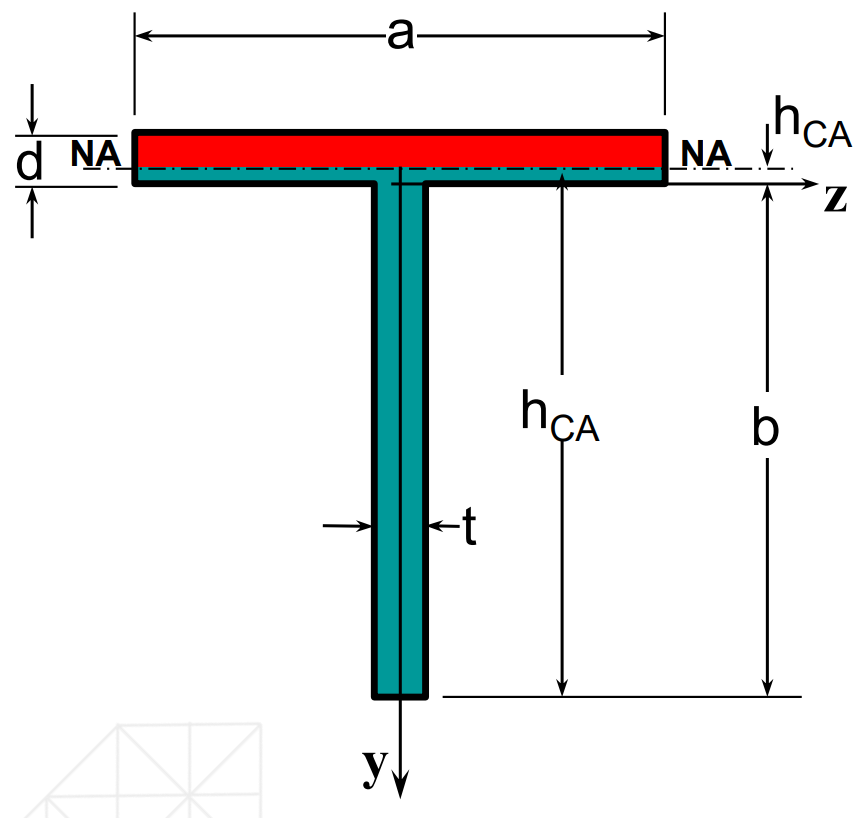
\includegraphics[width = 0.4 \textwidth]{../img/diagram6.PNG}
\end{figure}
\begin{gather}
  A_T = A_C = \frac{A_{total}}{2} \\[10pt]
  \text{Centre of Area} = h_{CA} = 0.72\text{mm}
\end{gather}
Where $A_T$ and $A_C$ represent the areas of the top and bottom parts.
\subsubsection{1st Moment of Area:}
\begin{figure}[H]
  \centering
  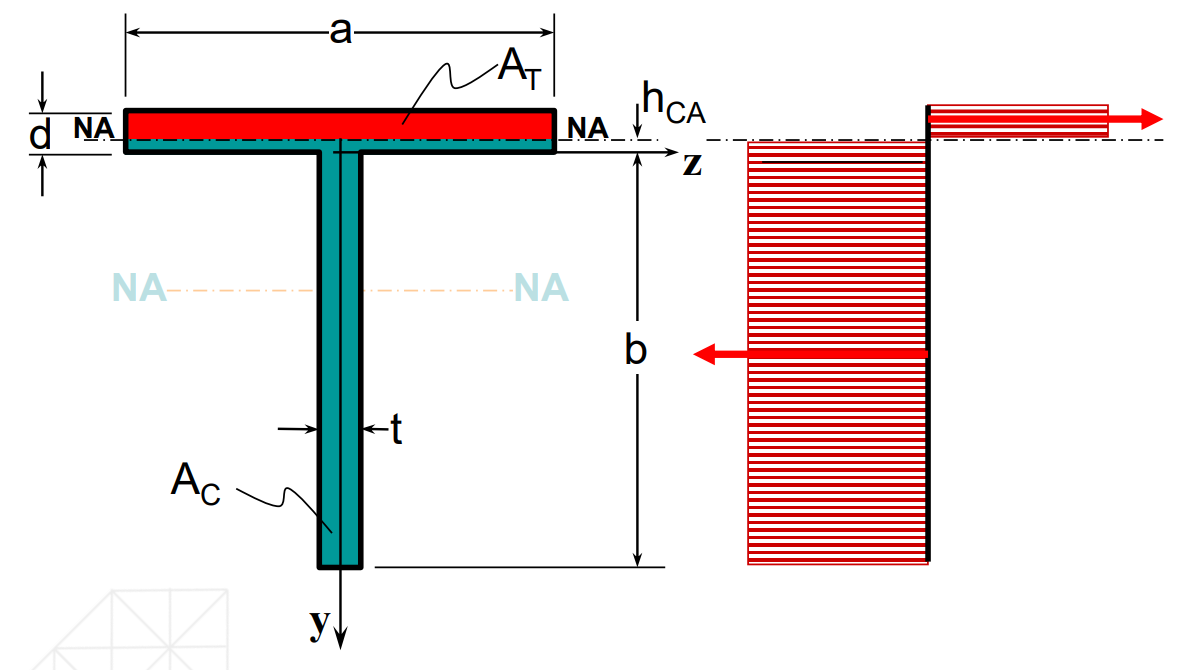
\includegraphics[width = 0.7 \textwidth]{../img/diagram7.PNG}
\end{figure}
1st moment of the areas in tension \& compression:
\begin{gather}
  Q_{A_T} = \int_{A_T}h\cdot\dif A = 6362\text{mm}^3 \\[10pt]
  Q_{A_C} = \int_{A_C}h\cdot\dif A = 46846\text{mm}^3
\end{gather}
\subsubsection{Plastic Moment:}
\begin{gather}
  M_P = \sigma_Y(Q_{A_T}+Q_{A_C}) = \sigma_Y\cdot 6362+\sigma_Y\cdot 46846 = 53208\cdot\sigma_Y
\end{gather}
\subsubsection{Shape Factor:}
Calculated yield and plastic moments:
\begin{gather}
  M_Y = \frac{\sigma_Y\cdot I_{zz}}{y_{CG}} = 29745\cdot\sigma_Y \\[10pt]
  M_P = \sigma_Y(Q_{A_T}+Q_{A_C}) = 53208\cdot\sigma_Y \\[10pt]
  \therefore \text{Shape Factor:}f=\frac{M_P}{M_Y} = 1.79
\end{gather}
\begin{figure}[H]
  \centering
  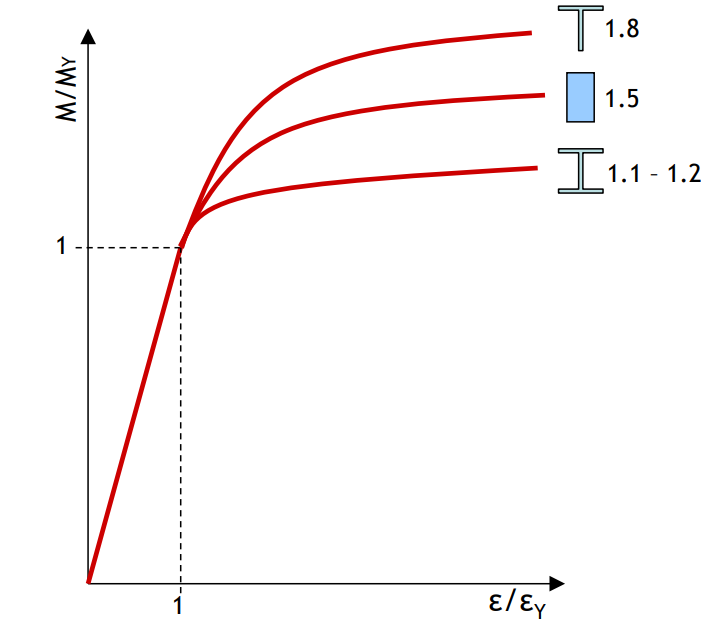
\includegraphics[width = 0.5 \textwidth]{../img/graph6.PNG}
  \caption{The shape factors of Rectangular, T-shaped and I-shaped cross sections}
\end{figure}
\end{document}